\subsubsection{模型建立}

针对问题一，从产销分段收益和跨期土地约束两个角度建立确定性多期MILP。

\textbf{步骤1 产量与销量线性化}

设$x_{tisj}$为年$t$季次$s$地块$i$种植作物$j$的面积，$z_{tisj}$为对应二元变量。该批次产量为
\begin{equation}
Y_{tisj}=y^0_{g_i s j}x_{tisj}.
\end{equation}
设$q_{tisj}$为按正常价格销售的产量，则
\begin{equation}
0\le q_{tisj}\le Y_{tisj},\qquad
\sum_{i,s}q_{tisj}\le D_j^0.
\end{equation}
当$\alpha=0$时超额产量滞销，当$\alpha=0.5$时超额部分按半价销售。七年目标函数为
\begin{equation}
\max \Pi^{(\alpha)}=
\sum_{t,i,s,j}\Bigl\{p^0_{g_i s j}\Bigl[\alpha y^0_{g_i s j}x_{tisj}+(1-\alpha)q_{tisj}\Bigr]-c^0_{g_i s j}x_{tisj}\Bigr\}.
\end{equation}

\textbf{步骤2 土地与管理约束}

地块容量和面积指示关系为
\begin{equation}
\sum_jx_{tisj}\le A_i,qquad
\rho A_i z_{tisj}\le x_{tisj}\le A_i z_{tisj},qquad
\sum_jz_{tisj}\le3.
\end{equation}
相邻可种植季内同一作物不能重茬。设$\mathcal B$为豆类集合，任意连续三年窗口满足
\begin{equation}
\sum_{\tau=t}^{t+2}\sum_s\sum_{j\in\mathcal B}x_{\tau isj}\ge A_i.
\end{equation}
水浇地模式变量保证水稻与两季蔬菜互斥，普通大棚、智慧大棚和露天地块均按题目适种规则建立变量。

\textbf{步骤3 求解设置}

模型使用HiGHS求解，并对两种管理配置进行比较。参数设置见表\ref{tab:q1_solver_setting}。

\begin{longtable}{>{\centering\arraybackslash}p{0.22\textwidth}>{\centering\arraybackslash}p{0.28\textwidth}>{\centering\arraybackslash}p{0.18\textwidth}>{\centering\arraybackslash}p{0.20\textwidth}}
  \caption{问题一求解参数设置}\label{tab:q1_solver_setting}\\
  \toprule
  参数 & 含义 & 取值 & 依据 \\
  \midrule
  \endfirsthead
  \caption{问题一求解参数设置（续）}\\
  \toprule
  参数 & 含义 & 取值 & 依据 \\
  \midrule
  \endhead
  \bottomrule
  \endfoot
  $\alpha$ & 超额销售折价 & 0，0.5 & 题目两种模式 \\
  $\rho$ & 最小面积占比 & 0，0.1 & 管理敏感性 \\
  $K$ & 每地块季次作物上限 & 3 & 人工管理配置 \\
  Gap & 滞销验收线 & 3\% & 人工确认 \\
  Gap & 半价验收线 & 1\% & 人工确认 \\
\end{longtable}

\subsubsection{模型求解}

正式滞销表采用$\rho=0$配置，累计净收益为4041.72万元，MIP Gap为2.126\%；正式半价销售表采用$\rho=0.1$配置，累计净收益为6351.02万元，MIP Gap为0.739\%。两份正式方案的硬约束违反数均为0。

两种销售规则下的收益比较如图\ref{fig:q1_profit}所示。半价销售允许超额产量继续产生收入，因此整体收益高于滞销模式。两种管理配置的收益差较小，说明10\%最小面积占比并未明显牺牲经济效益。
\begin{figure}[H]
  \centering
  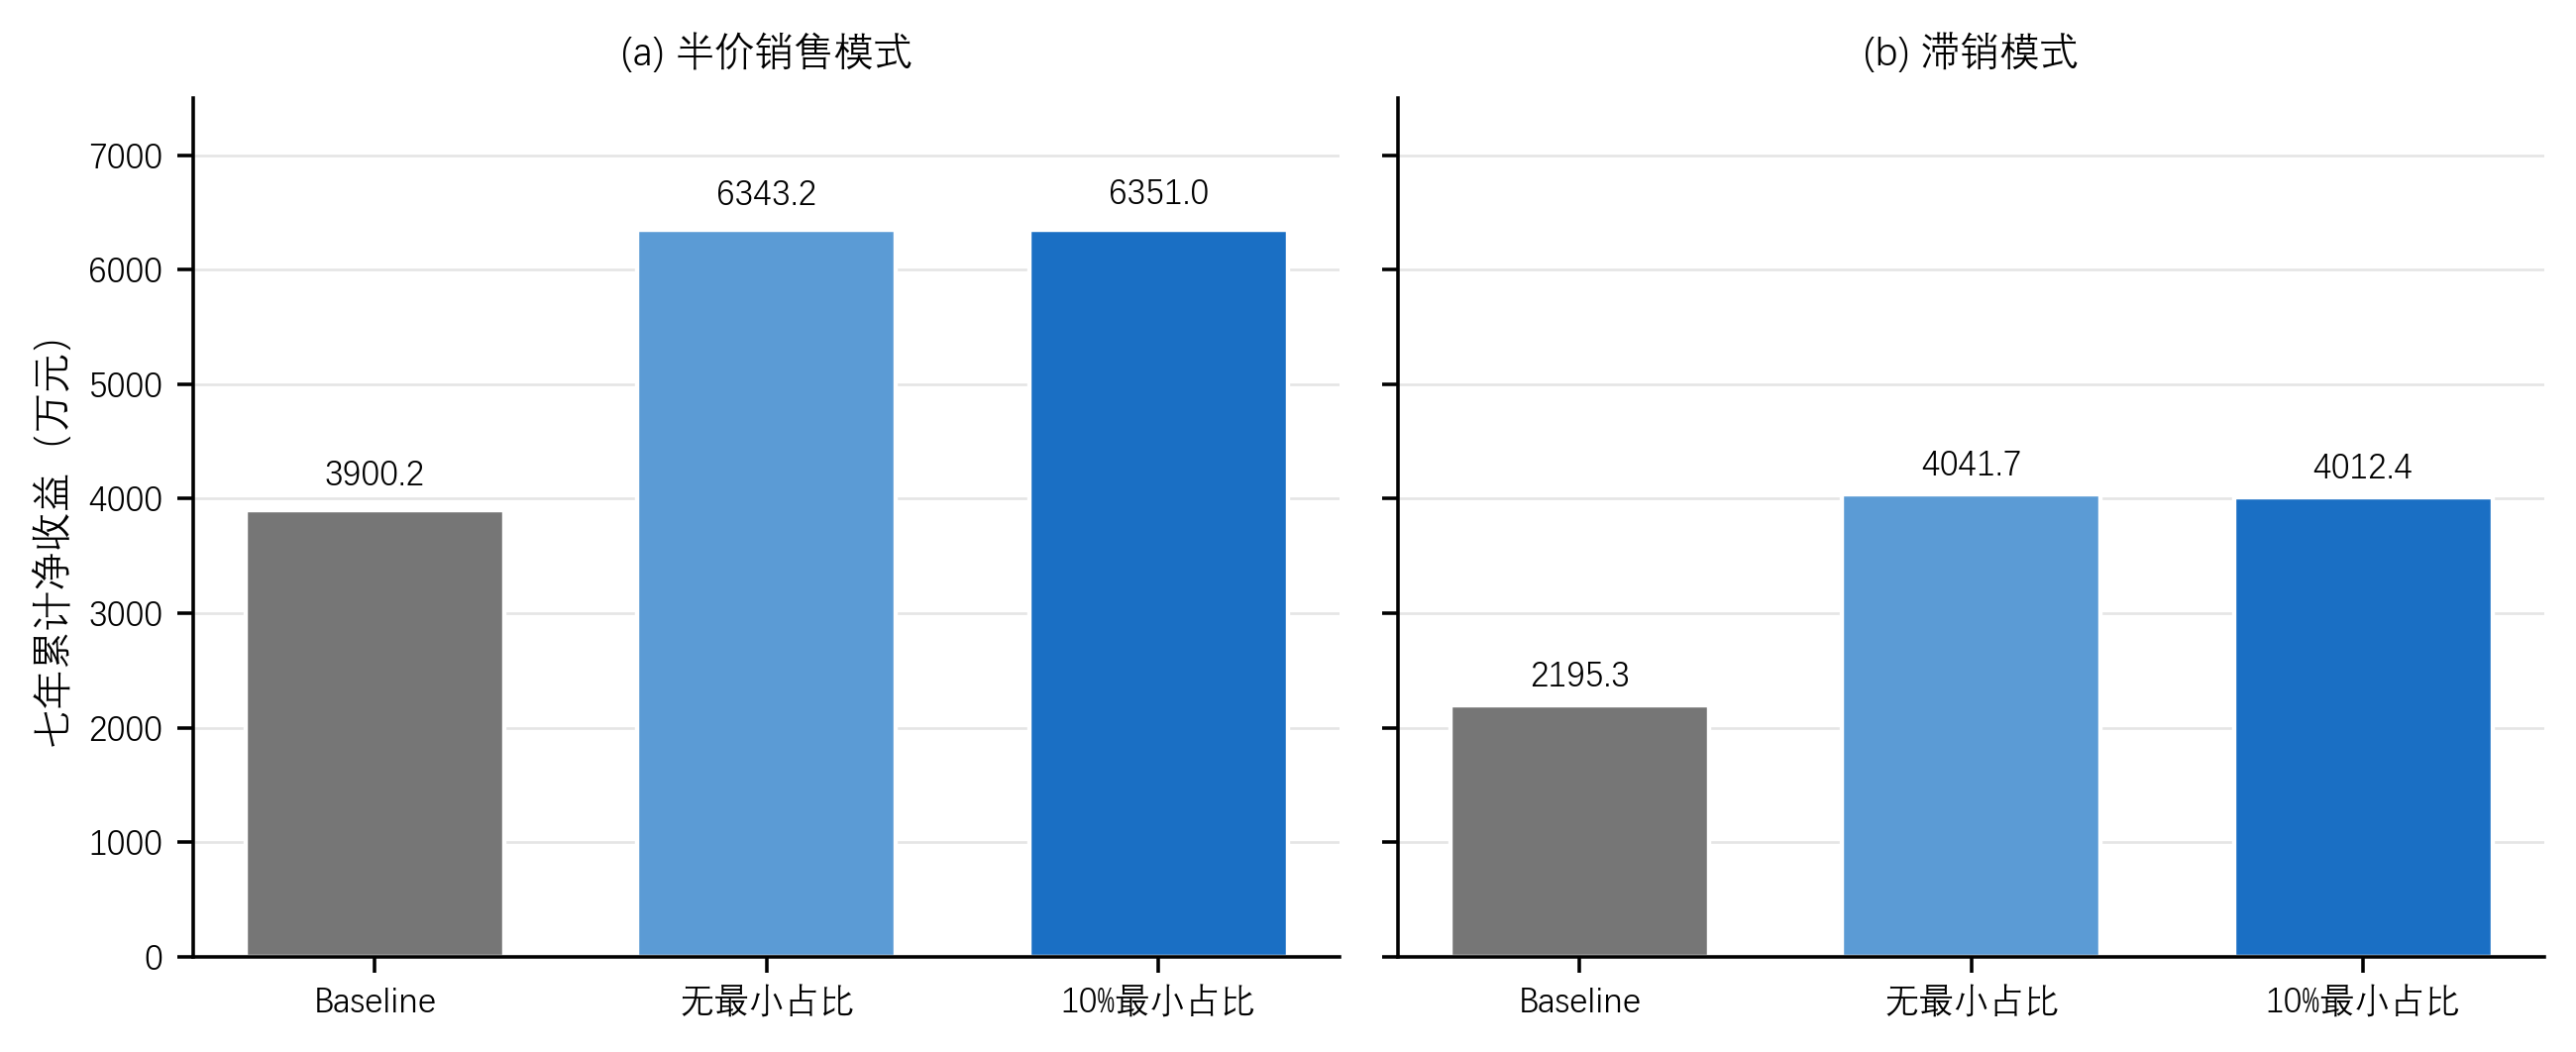
\includegraphics[width=0.96\textwidth]{figures/q1_cumulative_profit_comparison.png}
  \caption{问题一两种销售模式的七年累计净收益比较}
  \label{fig:q1_profit}
\end{figure}

\begin{longtable}{>{\centering\arraybackslash}p{0.15\textwidth}>{\centering\arraybackslash}p{0.16\textwidth}>{\centering\arraybackslash}p{0.17\textwidth}>{\centering\arraybackslash}p{0.12\textwidth}>{\centering\arraybackslash}p{0.10\textwidth}>{\centering\arraybackslash}p{0.10\textwidth}>{\centering\arraybackslash}p{0.08\textwidth}}
  \caption{问题一核心求解结果}\label{tab:q1_core}\\
  \toprule
  销售模式 & 配置 & 累计收益/万元 & Gap/\% & 作物数 & $H_3$/\% & 违反数 \\
  \midrule
  \endfirsthead
  \caption{问题一核心求解结果（续）}\\
  \toprule
  销售模式 & 配置 & 累计收益/万元 & Gap/\% & 作物数 & $H_3$/\% & 违反数 \\
  \midrule
  \endhead
  \bottomrule
  \endfoot
  半价销售 & 无最小占比 & 6343.21 & 0.864 & 24 & 44.88 & 0 \\
  半价销售 & 10\%最小占比 & 6351.02 & 0.739 & 24 & 42.10 & 0 \\
  滞销 & 无最小占比 & 4041.72 & 2.126 & 41 & 42.47 & 0 \\
  滞销 & 10\%最小占比 & 4012.39 & 2.869 & 41 & 41.87 & 0 \\
\end{longtable}

滞销正式方案仍保留2.126\%的未闭合最优间隙，因此只能表述为达到验收线的高质量可行解，不能称为精确全局最优。
